\documentclass[]{article}
\usepackage{lmodern}
\usepackage{amssymb,amsmath}
\usepackage{ifxetex,ifluatex}
\usepackage{fixltx2e} % provides \textsubscript
\ifnum 0\ifxetex 1\fi\ifluatex 1\fi=0 % if pdftex
  \usepackage[T1]{fontenc}
  \usepackage[utf8]{inputenc}
\else % if luatex or xelatex
  \ifxetex
    \usepackage{mathspec}
  \else
    \usepackage{fontspec}
  \fi
  \defaultfontfeatures{Ligatures=TeX,Scale=MatchLowercase}
\fi
% use upquote if available, for straight quotes in verbatim environments
\IfFileExists{upquote.sty}{\usepackage{upquote}}{}
% use microtype if available
\IfFileExists{microtype.sty}{%
\usepackage{microtype}
\UseMicrotypeSet[protrusion]{basicmath} % disable protrusion for tt fonts
}{}
\usepackage[margin=1in]{geometry}
\usepackage{hyperref}
\hypersetup{unicode=true,
            pdftitle={Characterizing cemented sandstones with physics-based and machine learning approaches},
            pdfauthor={Frank Male},
            pdfborder={0 0 0},
            breaklinks=true}
\urlstyle{same}  % don't use monospace font for urls
\usepackage{color}
\usepackage{fancyvrb}
\newcommand{\VerbBar}{|}
\newcommand{\VERB}{\Verb[commandchars=\\\{\}]}
\DefineVerbatimEnvironment{Highlighting}{Verbatim}{commandchars=\\\{\}}
% Add ',fontsize=\small' for more characters per line
\usepackage{framed}
\definecolor{shadecolor}{RGB}{248,248,248}
\newenvironment{Shaded}{\begin{snugshade}}{\end{snugshade}}
\newcommand{\KeywordTok}[1]{\textcolor[rgb]{0.13,0.29,0.53}{\textbf{#1}}}
\newcommand{\DataTypeTok}[1]{\textcolor[rgb]{0.13,0.29,0.53}{#1}}
\newcommand{\DecValTok}[1]{\textcolor[rgb]{0.00,0.00,0.81}{#1}}
\newcommand{\BaseNTok}[1]{\textcolor[rgb]{0.00,0.00,0.81}{#1}}
\newcommand{\FloatTok}[1]{\textcolor[rgb]{0.00,0.00,0.81}{#1}}
\newcommand{\ConstantTok}[1]{\textcolor[rgb]{0.00,0.00,0.00}{#1}}
\newcommand{\CharTok}[1]{\textcolor[rgb]{0.31,0.60,0.02}{#1}}
\newcommand{\SpecialCharTok}[1]{\textcolor[rgb]{0.00,0.00,0.00}{#1}}
\newcommand{\StringTok}[1]{\textcolor[rgb]{0.31,0.60,0.02}{#1}}
\newcommand{\VerbatimStringTok}[1]{\textcolor[rgb]{0.31,0.60,0.02}{#1}}
\newcommand{\SpecialStringTok}[1]{\textcolor[rgb]{0.31,0.60,0.02}{#1}}
\newcommand{\ImportTok}[1]{#1}
\newcommand{\CommentTok}[1]{\textcolor[rgb]{0.56,0.35,0.01}{\textit{#1}}}
\newcommand{\DocumentationTok}[1]{\textcolor[rgb]{0.56,0.35,0.01}{\textbf{\textit{#1}}}}
\newcommand{\AnnotationTok}[1]{\textcolor[rgb]{0.56,0.35,0.01}{\textbf{\textit{#1}}}}
\newcommand{\CommentVarTok}[1]{\textcolor[rgb]{0.56,0.35,0.01}{\textbf{\textit{#1}}}}
\newcommand{\OtherTok}[1]{\textcolor[rgb]{0.56,0.35,0.01}{#1}}
\newcommand{\FunctionTok}[1]{\textcolor[rgb]{0.00,0.00,0.00}{#1}}
\newcommand{\VariableTok}[1]{\textcolor[rgb]{0.00,0.00,0.00}{#1}}
\newcommand{\ControlFlowTok}[1]{\textcolor[rgb]{0.13,0.29,0.53}{\textbf{#1}}}
\newcommand{\OperatorTok}[1]{\textcolor[rgb]{0.81,0.36,0.00}{\textbf{#1}}}
\newcommand{\BuiltInTok}[1]{#1}
\newcommand{\ExtensionTok}[1]{#1}
\newcommand{\PreprocessorTok}[1]{\textcolor[rgb]{0.56,0.35,0.01}{\textit{#1}}}
\newcommand{\AttributeTok}[1]{\textcolor[rgb]{0.77,0.63,0.00}{#1}}
\newcommand{\RegionMarkerTok}[1]{#1}
\newcommand{\InformationTok}[1]{\textcolor[rgb]{0.56,0.35,0.01}{\textbf{\textit{#1}}}}
\newcommand{\WarningTok}[1]{\textcolor[rgb]{0.56,0.35,0.01}{\textbf{\textit{#1}}}}
\newcommand{\AlertTok}[1]{\textcolor[rgb]{0.94,0.16,0.16}{#1}}
\newcommand{\ErrorTok}[1]{\textcolor[rgb]{0.64,0.00,0.00}{\textbf{#1}}}
\newcommand{\NormalTok}[1]{#1}
\usepackage{graphicx,grffile}
\makeatletter
\def\maxwidth{\ifdim\Gin@nat@width>\linewidth\linewidth\else\Gin@nat@width\fi}
\def\maxheight{\ifdim\Gin@nat@height>\textheight\textheight\else\Gin@nat@height\fi}
\makeatother
% Scale images if necessary, so that they will not overflow the page
% margins by default, and it is still possible to overwrite the defaults
% using explicit options in \includegraphics[width, height, ...]{}
\setkeys{Gin}{width=\maxwidth,height=\maxheight,keepaspectratio}
\IfFileExists{parskip.sty}{%
\usepackage{parskip}
}{% else
\setlength{\parindent}{0pt}
\setlength{\parskip}{6pt plus 2pt minus 1pt}
}
\setlength{\emergencystretch}{3em}  % prevent overfull lines
\providecommand{\tightlist}{%
  \setlength{\itemsep}{0pt}\setlength{\parskip}{0pt}}
\setcounter{secnumdepth}{0}
% Redefines (sub)paragraphs to behave more like sections
\ifx\paragraph\undefined\else
\let\oldparagraph\paragraph
\renewcommand{\paragraph}[1]{\oldparagraph{#1}\mbox{}}
\fi
\ifx\subparagraph\undefined\else
\let\oldsubparagraph\subparagraph
\renewcommand{\subparagraph}[1]{\oldsubparagraph{#1}\mbox{}}
\fi

%%% Use protect on footnotes to avoid problems with footnotes in titles
\let\rmarkdownfootnote\footnote%
\def\footnote{\protect\rmarkdownfootnote}

%%% Change title format to be more compact
\usepackage{titling}

% Create subtitle command for use in maketitle
\providecommand{\subtitle}[1]{
  \posttitle{
    \begin{center}\large#1\end{center}
    }
}

\setlength{\droptitle}{-2em}

  \title{Characterizing cemented sandstones with physics-based and machine
learning approaches}
    \pretitle{\vspace{\droptitle}\centering\huge}
  \posttitle{\par}
    \author{Frank Male}
    \preauthor{\centering\large\emph}
  \postauthor{\par}
      \predate{\centering\large\emph}
  \postdate{\par}
    \date{04 October 2019}

\usepackage{amsmath}

\begin{document}
\maketitle

\subsection{Introduction}\label{introduction}

Sandstones one of the most common types of reservoir rocks. Let's see if
we can explain their permeability.

\subsection{Narrative}\label{narrative}

The most well-known physics-based approach to estimating permeability
was developed by Kozeny (1927) and later modified by Carman (1937). In
its modern form, the equation is written as

\begin{equation}
k = \frac{\phi^3}{2\tau(1-\phi)^2 a^2},
\end{equation}

which, for simplicity, we're going to recast as

\begin{equation}
k = \frac{\phi_{CK}}{2\tau a^2},
\end{equation}

where permeability is \(k\), porosity is \(\phi\), tortuosity is
\(\tau\), the specific surface area is \(a\), and the Carman-Kozeny void
fraction is \(\phi_{CK}\). For an uncemented sandstone, tortuosity can
be calculated following the derivation in Appendix B, which comes from
Panda and Lake (1994). For a cemented sandstone, the tortuosity changes
because of cements blocking and forcing modification of the flow paths.

Specific surface area for an uncemented sandstone can be estimated from
the particle size distribution, after assuming that the particles are
spherical. After cementation, the nature of the cement is important in
how the surface area changes. Some cements will coat the walls of the
pores, slightly decreasing the specific surface area. Other cements will
line or bridge the pores, moderately to greatly increasing the specific
surface area.

A competing hypothesis is that pore throat sizes are the most important
determinant of permeability-porosity transforms. This appears in the
Winland relations that follow the form

\begin{equation}
\log k = A \log \phi + B \log r + C,
\end{equation}

where \(r\) is the pore throat radius. Pore throat radius might be more
impacted by cements that coat the walls than cements that bridge the
pores. Wouldn't that be interesting?

Now, because this is a data-driven approach, let's start by comparing
permeability to the Carman-Kozeny void fraction.

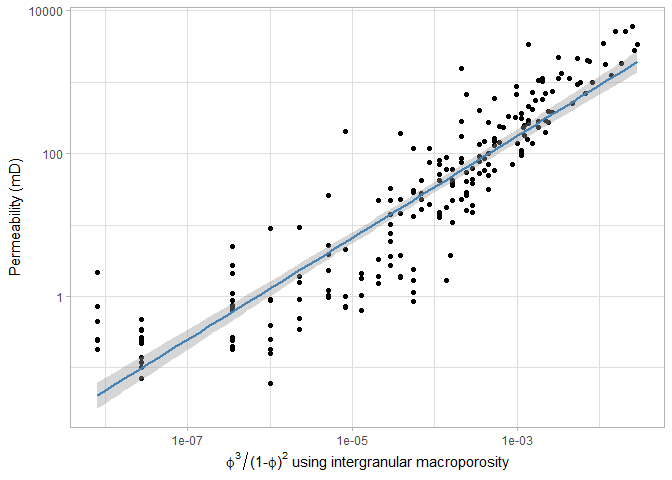
\includegraphics{garn-panda_files/figure-latex/CK_void_fraction-1.pdf}

\begin{verbatim}
## 
## Call:
## lm(formula = log(KLH) ~ log(CK_void_fraction), data = df)
## 
## Residuals:
##     Min      1Q  Median      3Q     Max 
## -3.2600 -0.8124  0.0698  0.7935  3.9761 
## 
## Coefficients:
##                       Estimate Std. Error t value Pr(>|t|)    
## (Intercept)           10.08803    0.24257   41.59   <2e-16 ***
## log(CK_void_fraction)  0.71222    0.02298   30.99   <2e-16 ***
## ---
## Signif. codes:  0 '***' 0.001 '**' 0.01 '*' 0.05 '.' 0.1 ' ' 1
## 
## Residual standard error: 1.261 on 213 degrees of freedom
## Multiple R-squared:  0.8185, Adjusted R-squared:  0.8176 
## F-statistic: 960.5 on 1 and 213 DF,  p-value: < 2.2e-16
\end{verbatim}

Hey! That's pretty good! The R\(^2\) is 0.85, and there are no odd
trends. Sure, at low porosity the data resolution starts to be a
problem, but that is at 1/100th of the average permeability, and ``the
permeability is bad'' is really all you need to know there. Okay, with
that positive result, let's add the grain size distribution to the model
and see if we can do even better. With the grain size, we can start
talking about the surface area of the pores. Bird et al. (1960) say that
permeability is related to the square of the pore radius, which is
roughly equivalent to the square of the grain diameter.

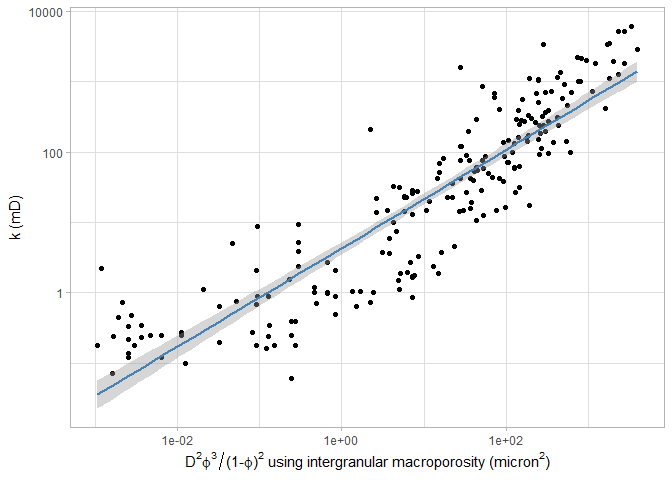
\includegraphics{garn-panda_files/figure-latex/CK_GS_porosity-1.pdf}

\begin{verbatim}
## 
## Call:
## lm(formula = log(KLH) ~ log(k_pred), data = mutate(df, k_pred = mean_GS^2 * 
##     CK_void_fraction))
## 
## Residuals:
##     Min      1Q  Median      3Q     Max 
## -3.2742 -0.8639  0.0866  0.8664  4.0401 
## 
## Coefficients:
##             Estimate Std. Error t value Pr(>|t|)    
## (Intercept)  1.45598    0.10427   13.96   <2e-16 ***
## log(k_pred)  0.69914    0.02359   29.64   <2e-16 ***
## ---
## Signif. codes:  0 '***' 0.001 '**' 0.01 '*' 0.05 '.' 0.1 ' ' 1
## 
## Residual standard error: 1.307 on 213 degrees of freedom
## Multiple R-squared:  0.8048, Adjusted R-squared:  0.8039 
## F-statistic: 878.5 on 1 and 213 DF,  p-value: < 2.2e-16
\end{verbatim}

Well, our Pearson correlation coefficent has gone down to 0.64. Nuts.
Well, it's pretty hard to estimate the mean grain size from looking at
Beard and Weyl's comparators, so I can understand that. Or\ldots{} how
well-sorted are these grains? Not that well-sorted? Then let's do a
specific surface area that takes that into account, with Panda and
Lake's derivation.

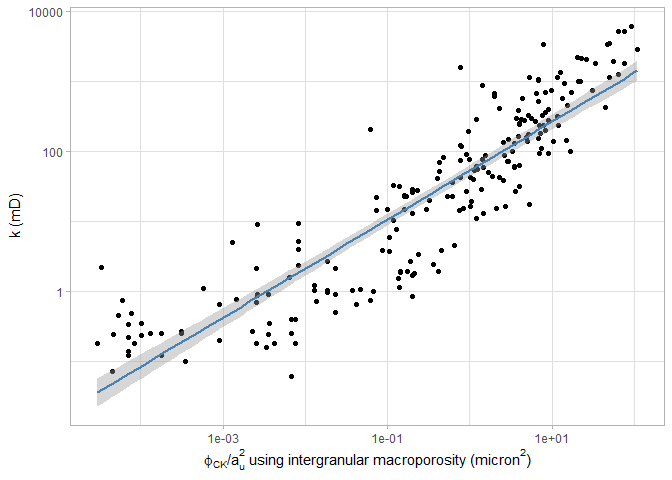
\includegraphics{garn-panda_files/figure-latex/CK_au_porosity-1.pdf}

\begin{verbatim}
## 
## Call:
## lm(formula = log(KLH) ~ log(k_pred), data = mutate(df, k_pred = CK_void_fraction/a_u^2))
## 
## Residuals:
##     Min      1Q  Median      3Q     Max 
## -3.2742 -0.8639  0.0866  0.8664  4.0401 
## 
## Coefficients:
##             Estimate Std. Error t value Pr(>|t|)    
## (Intercept)  3.96136    0.09422   42.05   <2e-16 ***
## log(k_pred)  0.69914    0.02359   29.64   <2e-16 ***
## ---
## Signif. codes:  0 '***' 0.001 '**' 0.01 '*' 0.05 '.' 0.1 ' ' 1
## 
## Residual standard error: 1.307 on 213 degrees of freedom
## Multiple R-squared:  0.8048, Adjusted R-squared:  0.8039 
## F-statistic: 878.5 on 1 and 213 DF,  p-value: < 2.2e-16
\end{verbatim}

Okay, so that's not helping the regression. It looks like Carman-Kozeny
void fraction is our best main predictor.

Maybe adding the uncemented tortuosity will help. Maybe both tortuosity
and the specific surface area are needed. Let's throw it all together,
then make a Spearman correlation table as well, for good measure.

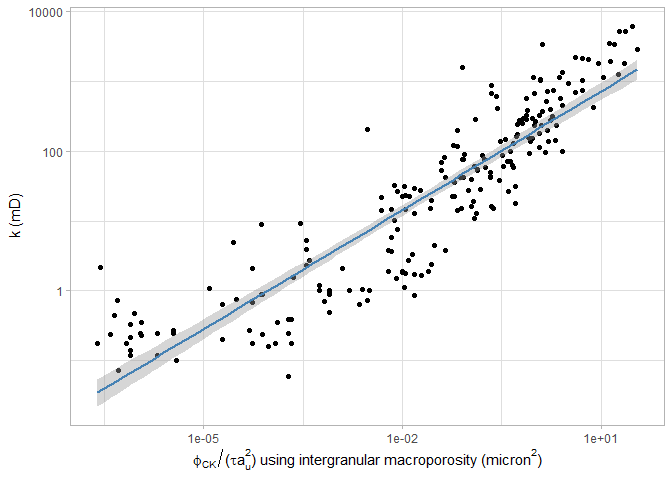
\includegraphics{garn-panda_files/figure-latex/CK_Av_tau-1.pdf}

\begin{verbatim}
## 
## Call:
## lm(formula = log(KLH) ~ log(k_pred), data = mutate(df, k_pred = CK_void_fraction/(tau_o * 
##     a_u^2)))
## 
## Residuals:
##     Min      1Q  Median      3Q     Max 
## -3.2216 -0.8336  0.0901  0.7968  4.0756 
## 
## Coefficients:
##             Estimate Std. Error t value Pr(>|t|)    
## (Intercept)   5.2586     0.1138   46.19   <2e-16 ***
## log(k_pred)   0.5662     0.0187   30.28   <2e-16 ***
## ---
## Signif. codes:  0 '***' 0.001 '**' 0.01 '*' 0.05 '.' 0.1 ' ' 1
## 
## Residual standard error: 1.285 on 213 degrees of freedom
## Multiple R-squared:  0.8115, Adjusted R-squared:  0.8106 
## F-statistic: 916.7 on 1 and 213 DF,  p-value: < 2.2e-16
\end{verbatim}

Okay, well, the original (pre-compaction) tortuosity is helping things.
Of course, it is a function of porosity, so really we're just building
more complicated models for explaining porosity's effect on
permeability. Also, this isn't really better than just using the
Carman-Kozeny void fraction. With that in mind, let's look at tortuosity
after taking the variable grain sizes into account.

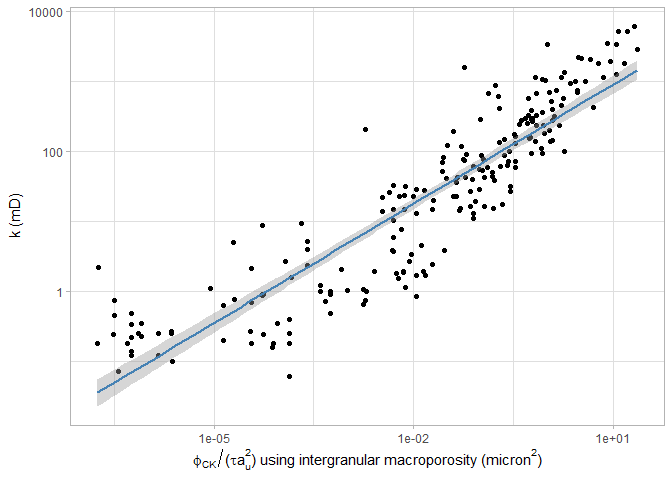
\includegraphics{garn-panda_files/figure-latex/CK_Av_tau_u-1.pdf}

\begin{verbatim}
## 
## Call:
## lm(formula = log(KLH) ~ log(k_pred), data = mutate(df, k_pred = CK_void_fraction/(tau_u * 
##     a_u^2)))
## 
## Residuals:
##     Min      1Q  Median      3Q     Max 
## -3.2422 -0.8158  0.1023  0.8130  4.1139 
## 
## Coefficients:
##             Estimate Std. Error t value Pr(>|t|)    
## (Intercept)   5.4844     0.1179   46.52   <2e-16 ***
## log(k_pred)   0.5676     0.0186   30.52   <2e-16 ***
## ---
## Signif. codes:  0 '***' 0.001 '**' 0.01 '*' 0.05 '.' 0.1 ' ' 1
## 
## Residual standard error: 1.277 on 213 degrees of freedom
## Multiple R-squared:  0.8139, Adjusted R-squared:  0.813 
## F-statistic: 931.6 on 1 and 213 DF,  p-value: < 2.2e-16
\end{verbatim}

And that helps a bit, but it still isn't as good as just using
\(\phi_{CK}\). But wait, there's more! Cementation should matter. Let's
try the cemented measure of tortuosity. That ought to get us somewhere.

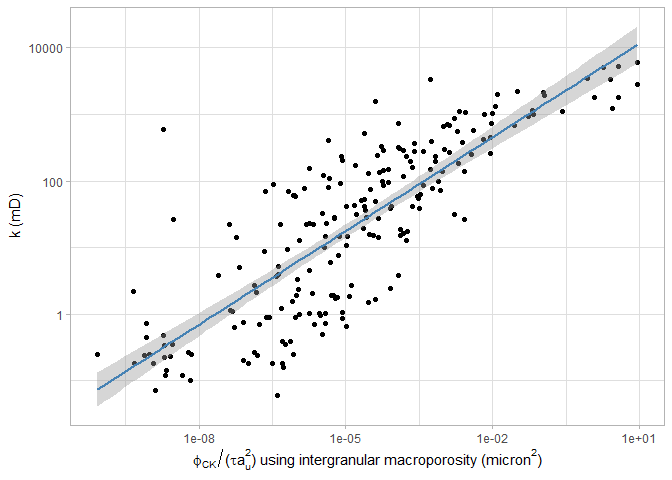
\includegraphics{garn-panda_files/figure-latex/cemented-1.pdf}

\begin{verbatim}
## 
## Call:
## lm(formula = log(KLH) ~ log(k_pred), data = mutate(df, k_pred = CK_void_fraction/(tau_e * 
##     a_u^2)))
## 
## Residuals:
##     Min      1Q  Median      3Q     Max 
## -4.1900 -1.1330 -0.0377  1.0642  7.5452 
## 
## Coefficients:
##             Estimate Std. Error t value Pr(>|t|)    
## (Intercept)  8.28334    0.27783   29.81   <2e-16 ***
## log(k_pred)  0.46949    0.02267   20.71   <2e-16 ***
## ---
## Signif. codes:  0 '***' 0.001 '**' 0.01 '*' 0.05 '.' 0.1 ' ' 1
## 
## Residual standard error: 1.705 on 213 degrees of freedom
## Multiple R-squared:  0.6681, Adjusted R-squared:  0.6665 
## F-statistic: 428.7 on 1 and 213 DF,  p-value: < 2.2e-16
\end{verbatim}

Oops, switching to effective tortuosity hurts the fit. Okay then, let's
add effective surface area. But how? The effective surface area has
fitting parameters that we don't know a priori --- the effects of pore
lining, bridging, and filling cement on the specific surface area. So,
what do we do? Well, let's start by looking at cement volume versus
permeability. Then, let's look at the Spearman correlation matrices
between these cements and permeability.

\begin{verbatim}
## `geom_smooth()` using method = 'loess' and formula 'y ~ x'
## `geom_smooth()` using method = 'loess' and formula 'y ~ x'
\end{verbatim}

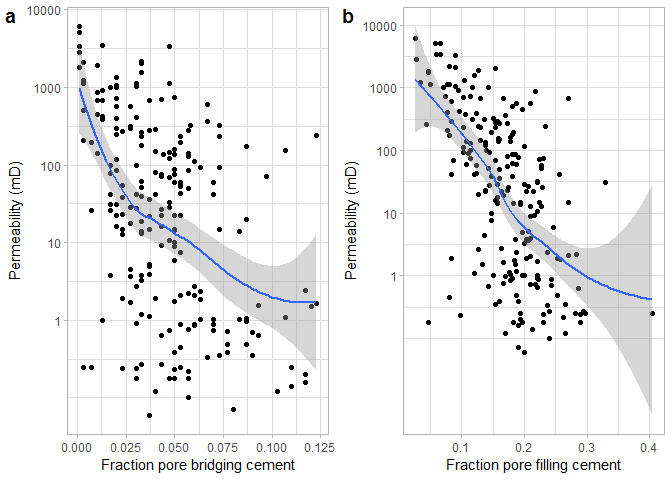
\includegraphics{garn-panda_files/figure-latex/unnamed-chunk-1-1.pdf}

\begin{verbatim}
##                  CK_void_fraction        P_b        P_f        KLH
## CK_void_fraction        1.0000000 -0.4197979 -0.5868664  0.9308890
## P_b                    -0.4197979  1.0000000  0.1151770 -0.4736764
## P_f                    -0.5868664  0.1151770  1.0000000 -0.6095451
## KLH                     0.9308890 -0.4736764 -0.6095451  1.0000000
\end{verbatim}

Ah ha! This matters. Nice, high, Spearman r values showing that
pore-filling and pore-bridging cement are bad for permeability. Now,
these also happen to be strongly correlated with interparticle porosity
and, as one might expect, so the story could be complicated, there. This
looks like enough to start setting up a regression. What form should
this regression take? Let's take some inspiration from Winland and
slightly abuse Panda and Lake's (1995) Carman-Kozeny equation.

After that abuse, the regression equation becomes

\begin{equation}
\log k = A_1 \log \phi_{CK} - A_2 \log P_b - A_3 \log P_f - A_4 \log a_u - A_5 \log \tau_e + A_0.
\end{equation}

Now, to the regressor!

\begin{verbatim}
## 
## Call:
## lm(formula = log(KLH) ~ log(CK_void_fraction) + log(P_b) + log(P_f) + 
##     log(a_u) + log(tau_e), data = df, na.action = na.exclude)
## 
## Residuals:
##     Min      1Q  Median      3Q     Max 
## -3.1513 -0.8064  0.0719  0.7716  3.8951 
## 
## Coefficients:
##                       Estimate Std. Error t value Pr(>|t|)    
## (Intercept)            5.01954    1.07582   4.666 5.49e-06 ***
## log(CK_void_fraction)  0.62982    0.02597  24.255  < 2e-16 ***
## log(P_b)              -0.46819    0.10312  -4.540 9.48e-06 ***
## log(P_f)              -0.77252    0.21598  -3.577 0.000432 ***
## log(a_u)              -0.11392    0.22681  -0.502 0.616002    
## log(tau_e)             0.07359    0.03829   1.922 0.055987 .  
## ---
## Signif. codes:  0 '***' 0.001 '**' 0.01 '*' 0.05 '.' 0.1 ' ' 1
## 
## Residual standard error: 1.157 on 209 degrees of freedom
## Multiple R-squared:  0.8499, Adjusted R-squared:  0.8463 
## F-statistic: 236.7 on 5 and 209 DF,  p-value: < 2.2e-16
\end{verbatim}

\begin{verbatim}
##      RMSE  Rsquared       MAE 
## 1.1410837 0.8499225 0.8866148
\end{verbatim}

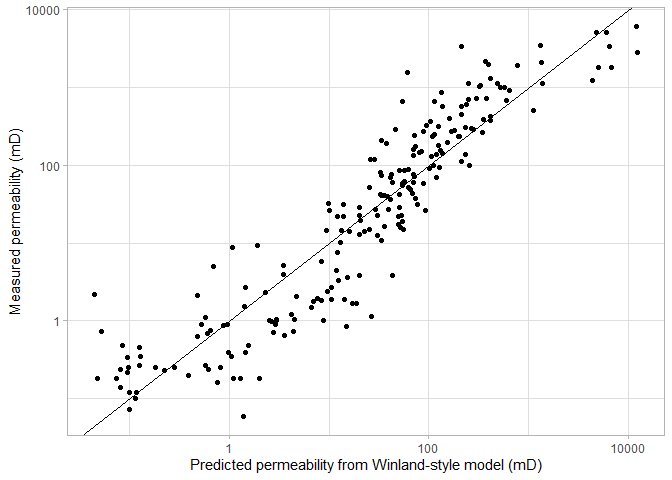
\includegraphics{garn-panda_files/figure-latex/cements_regression-1.pdf}

Now we're cooking with gas! An R\(^2\) of 0.87 is nothing to sneeze at.
Also, it's the first time we've improved beyond the straight
Carman-Kozeny void fraction relation. The one issue is that this assumes
a linear relationship between the cementation of various types and the
porosity. The solution here is to go to non-parametric fitting. Now,
non-parametric fitting is prone to overfitting, so we're going to have
to set up some cross-validation. After that, let's perform some
recursive feature elimination to figure out which features are really
impacting permeability. Then, let's use a gradient boosting regressor on
the significant features.

\begin{verbatim}
## [1] "The predictors are: CK_void_fraction, tau_e, P_f, P_b"
\end{verbatim}

This is not a terribly surprising result. Now, to the gradient boosting
regressor to see how it all comes together.

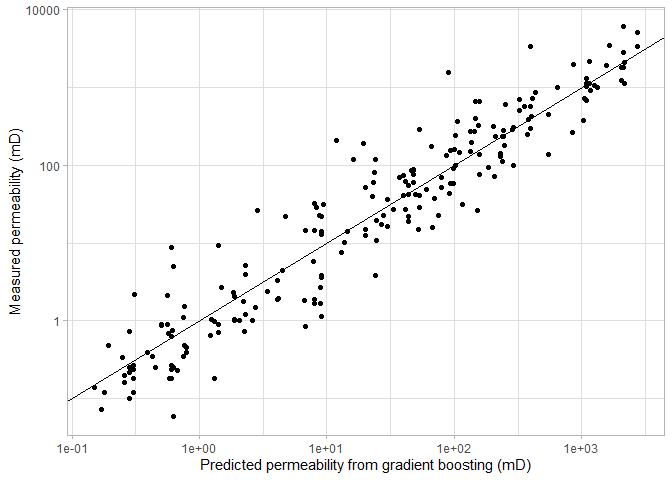
\includegraphics{garn-panda_files/figure-latex/unnamed-chunk-3-1.pdf}

\begin{verbatim}
##      RMSE  Rsquared       MAE 
## 3.3626574 0.7301831 2.9247083
\end{verbatim}

\begin{verbatim}
##      RMSE  Rsquared       MAE 
## 5.2617136 0.5800722 4.9913699
\end{verbatim}

\begin{verbatim}
## 
## Attaching package: 'xgboost'
\end{verbatim}

\begin{verbatim}
## The following object is masked from 'package:dplyr':
## 
##     slice
\end{verbatim}

\begin{verbatim}
## Scale for 'x' is already present. Adding another scale for 'x', which
## will replace the existing scale.
\end{verbatim}

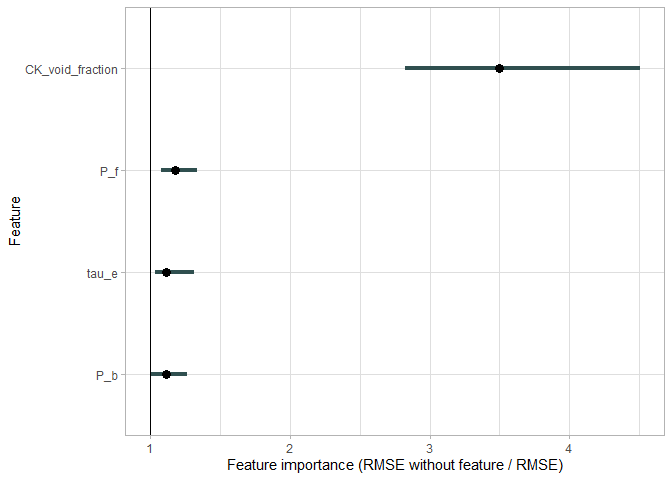
\includegraphics{garn-panda_files/figure-latex/varImp-1.pdf}
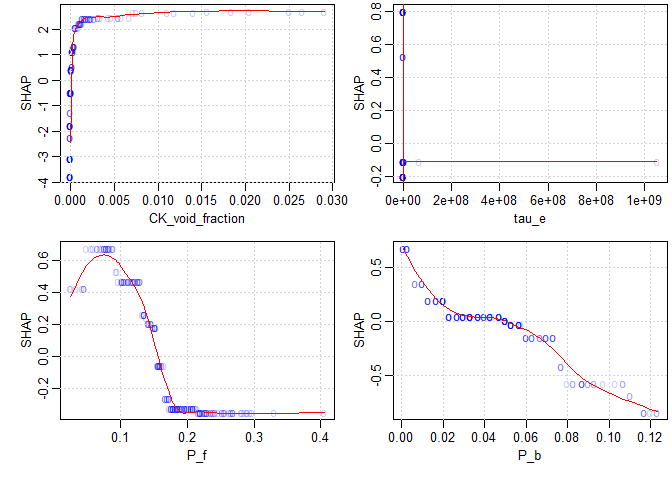
\includegraphics{garn-panda_files/figure-latex/varImp-2.pdf}
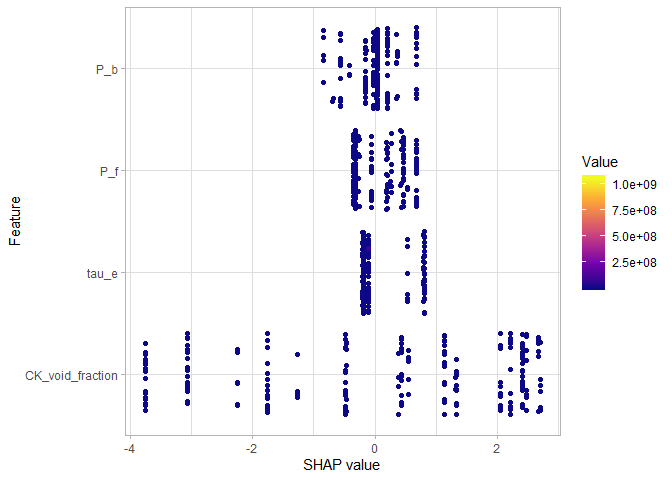
\includegraphics{garn-panda_files/figure-latex/varImp-3.pdf}
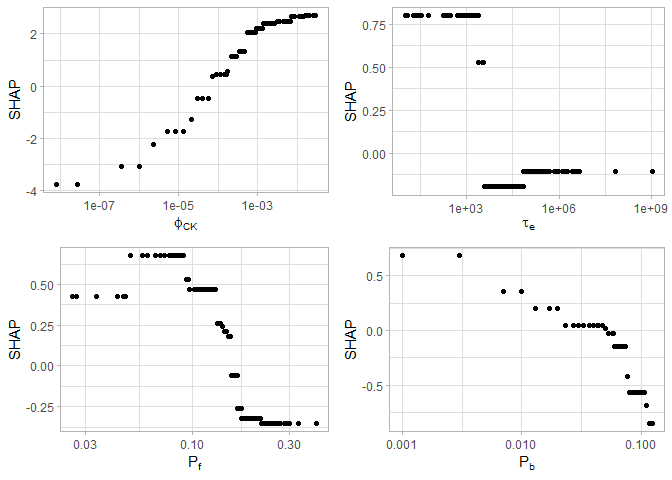
\includegraphics{garn-panda_files/figure-latex/varImp-4.pdf}

\subsection{Appendix A}\label{appendix-a}

\subsubsection{Derivation of a modified Carman-Kozeny equation for
uncemented
sandstones}\label{derivation-of-a-modified-carman-kozeny-equation-for-uncemented-sandstones}

\paragraph{Following Panda and Lake
(1994)}\label{following-panda-and-lake-1994}

We start with the Carman-Kozeny equation

\begin{equation}
k = \frac{\phi^3}{2\tau(1-\phi)^2 a^2},
\end{equation}

where permeability is \(k\), porosity is \(\phi\), tortuosity is
\(\tau\), and the specific surface area is \(a\). For porosity, we use
the porosity to Helium that has been measured on the Garn data.
Permeability is air permeability that has been corrected for Klinkenberg
effects. In order to measure tortuosity and specific surface area, we
have measurements of the median grain size and Trask sorting
coefficient, following the approach proposed by Beard and Weyl (1973).
Skewness of the distribution of grain sizes can be extracted from these
parameters.

Given this information, a modified Carman Kozeny equation following
Panda and Lake (1994) is

\begin{equation}
k = \frac{\bar{D}^2 \phi^3}{72\tau_u \left(1-\phi \right)^2} \frac{\left(\gamma C_D^3 + 3C_D^2 +1 \right)^2}{\left(1+C_D^2\right)^2},
\end{equation}

where \(\bar{D}\) is the mean particle size, \(C_D\) is the coefficient
of varation of the particle size distribution
(\(C_D=\sigma_D/\bar{D}\)), \(\gamma\) is the skewness of the particle
size distribution. and \(\tau_u\) is the tortuosity of an
unconsolidated, uncemented sand.

Panda and Lake (1994) do not calculate the original tortuosity. However,
there has been a wealth of work on this problem in the physics, soil,
and petroleum literature. One approach is proposed by Ghanbarian, et al.
(2013). This approach makes use of percolation theory and results in
tortuosity following a power law with respect to porosity. Taking their
equation 8 (which assumes reasonably well-sorted grains and a large
system) and plugging in the relevant numbers, original tortuosity
follows the equation

\begin{align}
\tau_o &= \left(\frac{\phi - \phi_t}{1 - \phi_t} \right)^{\nu(1-D)} \\
 &= \left(\frac{0.9\phi}{1-0.1\phi} \right)^{-0.378}
\end{align}

Panda and Lake (1995) use a surface area argument to derive the
effective tortuosity for an uncemented sandstone of different size
particles, which is

\begin{equation}
\tau_u = \tau_o \left(1 + C_D^2 \right).
\end{equation}

Next, let's look at the distribution of the distribution measures,
\(\bar D,\ C_D\), and \(\gamma\):
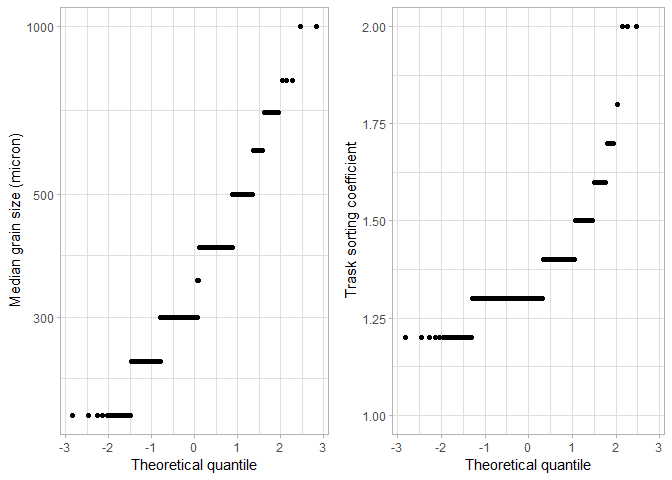
\includegraphics{garn-panda_files/figure-latex/distribution-1.pdf}
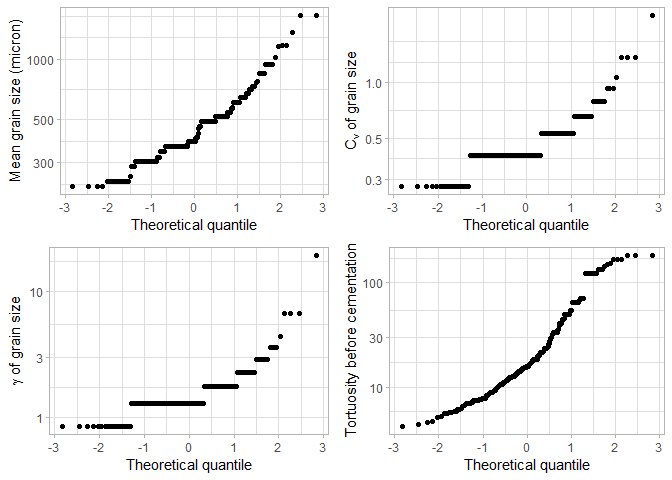
\includegraphics{garn-panda_files/figure-latex/distribution-2.pdf}

\subsection{Appendix B}\label{appendix-b}

\subsubsection{Derivation of Carman-Kozeny corrections for cemented
sandstones}\label{derivation-of-carman-kozeny-corrections-for-cemented-sandstones}

\paragraph{Following Panda and Lake
(1995)}\label{following-panda-and-lake-1995}

Carman-Kozeny theory does not consider the effect of cementation on
permeability, but we know that cement is present in these rocks, and
that it blocks flow paths, decreasing the permeability. In terms of the
quantities considered by Carman and Kozeny, this changes the tortuosity
and the specific surface area. There are several different cements that
could be present, and they are measured through point counting. The next
figure shows the abundance of each cement.

\begin{verbatim}
## No id variables; using all as measure variables
\end{verbatim}

\begin{verbatim}
## Picking joint bandwidth of 0.689
\end{verbatim}

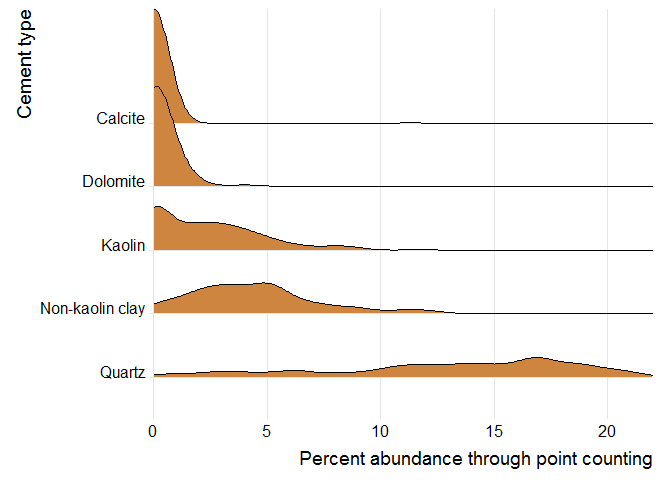
\includegraphics{garn-panda_files/figure-latex/cements-1.pdf}

Panda and Lake (1995) separate cement types into three categories:
pore-filling, pore-lining, and pore-briding, following Neasham (1997).
Where cements associate with the pores depends on the thermodynamic
properties of the cementing material. Crystal-like kaolinite and dickite
cements are pore-filling. Other pore-filling cements include quartz,
feldspar, dolomite, and calcite. These cements affect the porosity, but
because they do not affect the pore throats or the pore shape, they have
a small effect on permeability.

Pore-lining cements find it energetically favorable to form long
crystals that stretch out from the grains. These cements include the
non-kaolinite clay minerals, such as chlorite, illite, and smectite. The
long crystals affect permeability more than they affect porosity because
of the large surface areas they generate.

Pore-bridging cements can partially or completely block the pore
throats. This strongly influences the permeability, increasing the
tortuosity of the system and decreasing the connectivity. Examples of
the minerals that bridge pores include illite, chlorite, and
montmorillonite (the non-Kaolin clay minerals).

After cementation, the tortuosity and specific surface area has changed.
Panda and Lake (1995) suggest an effective tortuosity, \(\tau_e\), given
by

\begin{equation}
\tau_e = \tau_u \left(1+C_D^2 \right)\left(1+\frac{Rm_b}{1-m_b} \right)^2 \left(1 + \frac{2m}{(1-m) \phi^{1/3}} \right)^2,
\end{equation}

where \(R\) is a constant equal to 2 indicating the additional distance
traveled by the fluid as a function of the thickness of cementation. The
volume fraction of pore-bridging cement is \(m_b = P_b(1-\phi)/\phi\),
and the volume fraction of pore-filling cement is
\(m = P_f (1-\phi)/\phi\).

For an unconsolidated sand of variable sizes, the specific surface area
is

\begin{equation}
a_u = \frac{6(\sigma^2 + \bar{D}^2)}{\gamma \sigma^3 + 3\bar{D}\sigma^2 + \bar{D}^3}
\end{equation}

After cementation, the effective specific surface area follows the
equation

\begin{equation}
a_e = a_u \frac{1-\phi_u}{1-\phi} + a_b P_b + a_f P_f
\end{equation}

where \(a_u\) is the specific surface area for an unconsolidated,
uncemented sand, \(\phi_u\) is the porosity of an unconsolidated sand,
\(a_b\) is the specific surface area for a pore-bridging cement, \(a_f\)
is the specific surface area for a pore-filling cement, and \(P_b,P_f\)
are the relative fractions of pore-bridging and pore-filling cement,
respectively.

Taking these equations together, the equation for permeability becomes

\begin{equation}
k = \left[\bar{D}^2 \phi^3 \left(\gamma C_D^3 + 3C_D^2 + 1 \right)^2 \right]
 \left\{ 2\tau_e (1-\phi)^2 \left[ 6\left(1+C_D^2 \right) \frac{1-\phi_u}{1-\phi} + 
 \left(a_b P_b + a_f P_f \right) \bar{D} \left(\gamma C_D^3 + 3C_D^2 +1 \right) \right]^2\right\}^{-1}
\end{equation}

Now, with these calculations, the properties of the grain size
distribution measured by Ehrenberg (1990) can be used to test the theory
derived by Panda and Lake (1995).

First, let's look at the distributions of tortuosity and effective
specific surface area.

\subsection{Appendix C}\label{appendix-c}

\subsubsection{Lognormal distribution
statistics}\label{lognormal-distribution-statistics}

Here we relate median grain size and the Trask Sorting Coefficient
(\(S_o\)) to the mean, standard deviation, and skewness of the grain
size distribution. From the mean and standard deviation, the coefficient
of variation, \(C_v = \bar{D}/\sigma\), can be calculated.

Grain size distribution is often described by the median grain size and
the Trask Sorting Coefficient (\(S_o\)), which is defined by
\(S_o=\sqrt{D_{0.75}/D_{0.25}}\), where \(D_p\) is the quantile value
indicated by \(p\), such that \(D_{0.25}\) is the 25\%-ile grain size.
Panda (1994, Appendix B) derived an equation relating average grain
size, Trask Sorting Coefficient, and the standard deviation of the grain
size, which is

\begin{equation}
\sigma = \bar{D} \frac{S_o^2-1}{0.675\left(S_o^2+1\right)}.
\end{equation}

This equation is done through \(D_p\) being calculated in a \(\log_2\)
space, but most calculations of \(S_o\) use the definition I provided
above, so this should be re-derived.

According to my derivation, assuming lognormality, following a
distribution with the PDF

\begin{equation}
\frac{1}{x\sigma\sqrt{2\pi}} \exp\left(-\frac{(\ln x-\mu)^2}{2\sigma^2} \right),
\end{equation}

the mean grain size is \(\bar{D} = \exp(\mu + \sigma/2)\), and in terms
of the median and Trask sorting coefficient, the parameters of the
distribution are

\begin{align}
\mu &= \ln D_{0.5}\\
\sigma &= \frac{\ln S_o}{\sqrt{2}\ \text{erf}^{-1}(0.5)}
\end{align}

Okay, let's test those stats with a randomly generated lognormal
distribution:

\begin{Shaded}
\begin{Highlighting}[]
\NormalTok{mu <-}\StringTok{ }\FloatTok{3.14159}
\NormalTok{sigma <-}\StringTok{ }\DecValTok{1}
\NormalTok{d <-}\StringTok{ }\KeywordTok{rlnorm}\NormalTok{(}\DecValTok{10000}\NormalTok{, mu, sigma) }\CommentTok{# distribution of 1k points with mu=10, sigma=1}

\NormalTok{trask <-}\StringTok{ }\KeywordTok{sqrt}\NormalTok{(}\KeywordTok{quantile}\NormalTok{(d,}\FloatTok{0.75}\NormalTok{) }\OperatorTok{/}\StringTok{ }\KeywordTok{quantile}\NormalTok{(d,}\FloatTok{0.25}\NormalTok{))}
\NormalTok{d_}\DecValTok{50}\NormalTok{ <-}\StringTok{ }\KeywordTok{median}\NormalTok{(d)}
\NormalTok{mu_calc <-}\StringTok{ }\KeywordTok{log}\NormalTok{(d_}\DecValTok{50}\NormalTok{)}
\NormalTok{erfinv <-}\StringTok{ }\ControlFlowTok{function}\NormalTok{(x) }\KeywordTok{qnorm}\NormalTok{((x }\OperatorTok{+}\StringTok{ }\DecValTok{1}\NormalTok{)}\OperatorTok{/}\DecValTok{2}\NormalTok{)}\OperatorTok{/}\KeywordTok{sqrt}\NormalTok{(}\DecValTok{2}\NormalTok{)}
\NormalTok{sigma_calc <-}\StringTok{ }\KeywordTok{log}\NormalTok{(trask) }\OperatorTok{/}\StringTok{ }\NormalTok{(}\KeywordTok{sqrt}\NormalTok{(}\DecValTok{2}\NormalTok{) }\OperatorTok{*}\StringTok{ }\KeywordTok{erfinv}\NormalTok{(}\FloatTok{0.5}\NormalTok{))}
\NormalTok{mean_calc <-}\StringTok{ }\KeywordTok{exp}\NormalTok{(}\KeywordTok{log}\NormalTok{(d_}\DecValTok{50}\NormalTok{) }\OperatorTok{+}\StringTok{ }\NormalTok{sigma_calc}\OperatorTok{/}\DecValTok{2}\NormalTok{)}
\NormalTok{exponent_thingie <-}\StringTok{ }\NormalTok{(}\DecValTok{2}\OperatorTok{*}\KeywordTok{sqrt}\NormalTok{(}\DecValTok{2}\NormalTok{) }\OperatorTok{*}\StringTok{ }\KeywordTok{erfinv}\NormalTok{(}\FloatTok{0.5}\NormalTok{))}

\KeywordTok{cat}\NormalTok{(}
  \StringTok{"}\CharTok{\textbackslash{}n}\StringTok{The median is"}\NormalTok{, }\KeywordTok{round}\NormalTok{(}\KeywordTok{median}\NormalTok{(d),}\DecValTok{1}\NormalTok{),}
       \StringTok{"It should be"}\NormalTok{, }\KeywordTok{round}\NormalTok{(}\KeywordTok{exp}\NormalTok{(mu),}\DecValTok{1}\NormalTok{),}
      \StringTok{"}\CharTok{\textbackslash{}n}\StringTok{The mean is"}\NormalTok{,}\KeywordTok{round}\NormalTok{(}\KeywordTok{mean}\NormalTok{(d),}\DecValTok{1}\NormalTok{),}
      \StringTok{"It should be"}\NormalTok{, }\KeywordTok{round}\NormalTok{(}\KeywordTok{exp}\NormalTok{(mu }\OperatorTok{+}\StringTok{ }\NormalTok{sigma}\OperatorTok{/}\DecValTok{2}\NormalTok{),}\DecValTok{1}\NormalTok{),}
      \StringTok{"}\CharTok{\textbackslash{}n}\StringTok{The standard deviation is"}\NormalTok{,}\KeywordTok{round}\NormalTok{(}\KeywordTok{sd}\NormalTok{(d),}\DecValTok{1}\NormalTok{),}
      \StringTok{"It should be"}\NormalTok{,}\KeywordTok{round}\NormalTok{( }\KeywordTok{sqrt}\NormalTok{( (}\KeywordTok{exp}\NormalTok{(sigma}\OperatorTok{^}\DecValTok{2}\NormalTok{)}\OperatorTok{-}\DecValTok{1}\NormalTok{) }\OperatorTok{*}\StringTok{ }\KeywordTok{exp}\NormalTok{(}\DecValTok{2}\OperatorTok{*}\NormalTok{mu}\OperatorTok{+}\NormalTok{sigma}\OperatorTok{^}\DecValTok{2}\NormalTok{))),}
      \StringTok{"}\CharTok{\textbackslash{}n}\StringTok{The Trask sorting coefficient is"}\NormalTok{,}\KeywordTok{round}\NormalTok{(}\KeywordTok{sqrt}\NormalTok{(}\KeywordTok{quantile}\NormalTok{(d,}\FloatTok{0.75}\NormalTok{) }\OperatorTok{/}\StringTok{ }\KeywordTok{quantile}\NormalTok{(d,}\FloatTok{0.25}\NormalTok{)),}\DecValTok{2}\NormalTok{),}
  \StringTok{"}\CharTok{\textbackslash{}n}\StringTok{From the Trask and median diameters, the mean should be"}\NormalTok{, }\KeywordTok{round}\NormalTok{(mean_calc,}\DecValTok{1}\NormalTok{),}\StringTok{"or"}\NormalTok{,}
  \KeywordTok{round}\NormalTok{(d_}\DecValTok{50} \OperatorTok{*}\StringTok{ }\NormalTok{trask}\OperatorTok{^}\NormalTok{(}\DecValTok{1}\OperatorTok{/}\NormalTok{(}\DecValTok{2}\OperatorTok{*}\KeywordTok{sqrt}\NormalTok{(}\DecValTok{2}\NormalTok{) }\OperatorTok{*}\StringTok{ }\KeywordTok{erfinv}\NormalTok{(}\FloatTok{0.5}\NormalTok{))),}\DecValTok{1}\NormalTok{),}
  \StringTok{"}\CharTok{\textbackslash{}n}\StringTok{This is a deviation of"}\NormalTok{, }\KeywordTok{round}\NormalTok{((}\KeywordTok{exp}\NormalTok{(mu }\OperatorTok{+}\StringTok{ }\NormalTok{sigma}\OperatorTok{/}\DecValTok{2}\NormalTok{) }\OperatorTok{-}\StringTok{ }\NormalTok{mean_calc)}\OperatorTok{/}\KeywordTok{exp}\NormalTok{(mu }\OperatorTok{+}\StringTok{ }\NormalTok{sigma}\OperatorTok{/}\DecValTok{2}\NormalTok{)}\OperatorTok{*}\DecValTok{100}\NormalTok{,}\DecValTok{1}\NormalTok{),}\StringTok{"percent}\CharTok{\textbackslash{}n}\StringTok{"}
      
\NormalTok{)}
\end{Highlighting}
\end{Shaded}

\begin{verbatim}
## 
## The median is 23.4 It should be 23.1 
## The mean is 37.8 It should be 38.2 
## The standard deviation is 48.2 It should be 50 
## The Trask sorting coefficient is 1.95 
## From the Trask and median diameters, the mean should be 38.4 or 38.4 
## This is a deviation of -0.6 percent
\end{verbatim}

The mean grain size can be calculated from the median grain size and
standard deviation through the equation (assuming a lognormal
distribution of the grain size). In addition, the coefficient of
variation and skewness can be calculated. The equations for these terms
are

\begin{align}
\bar{D} &= \exp \left[ \ln(D_{\text{0.5}}) + \sigma/2 \right] 
        &= D_{0.5} S_o^{1/{(2\sqrt{2}\ \text{erf}^{-1}(0.5)})} 
        &= D_{0.5} S_o^{1.349}\\
C_D &= \sqrt{e^{\sigma^2}-1} 
    &= \sqrt{e^{2.198(\ln S_o)^2} -1} & \\
\gamma &= \left(e^{\sigma^2} + 2\right) \sqrt{e^{\sigma^2}-1} 
       &= \left(e^{\sigma^2} + 2\right) C_D 
       &= \left( e^{2.198(\ln S_o)^2} + 2\right)\sqrt{e^{2.198(\ln S_o)^2} -1}
\end{align}

\section{ETC}\label{etc}

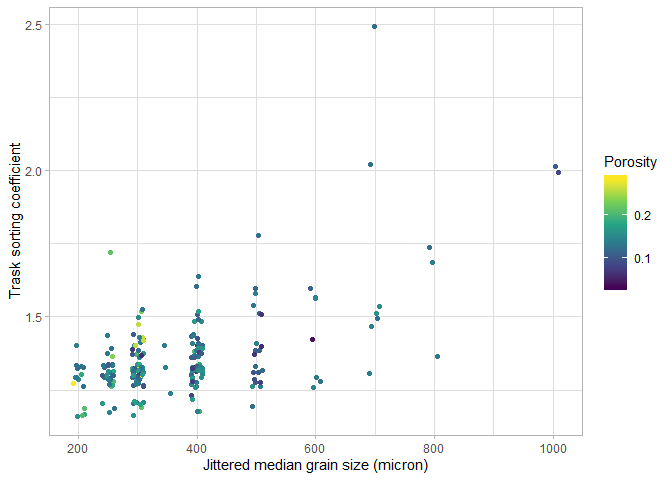
\includegraphics{garn-panda_files/figure-latex/eda-1.pdf}

\begin{verbatim}
## `stat_bin()` using `bins = 30`. Pick better value with `binwidth`.
\end{verbatim}

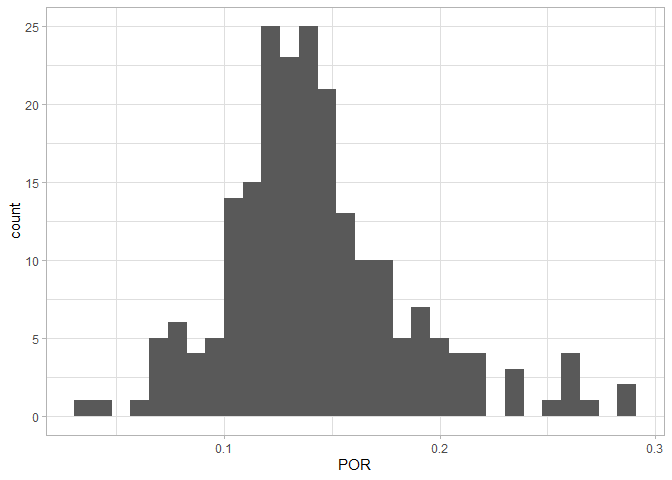
\includegraphics{garn-panda_files/figure-latex/eda-2.pdf}
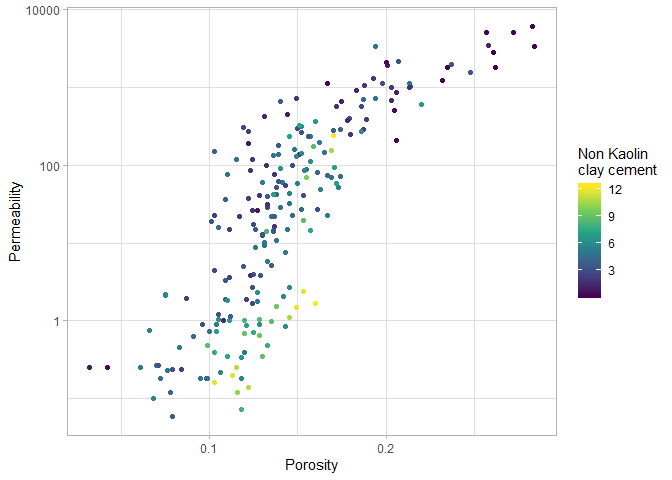
\includegraphics{garn-panda_files/figure-latex/eda-3.pdf}

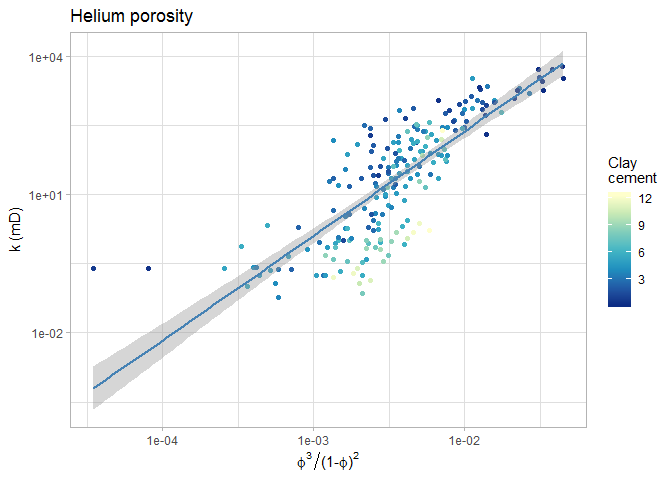
\includegraphics{garn-panda_files/figure-latex/Carman_Kozeny_unaltered-1.pdf}

\begin{verbatim}
## 
## Call:
## lm(formula = KLH ~ POR^3/(1 - POR)^2, data = df)
## 
## Residuals:
##     Min      1Q  Median      3Q     Max 
## -1030.6  -321.9  -128.0   191.1  3731.1 
## 
## Coefficients:
##             Estimate Std. Error t value Pr(>|t|)    
## (Intercept)  -1688.4      138.1  -12.22   <2e-16 ***
## POR          14199.0      926.1   15.33   <2e-16 ***
## ---
## Signif. codes:  0 '***' 0.001 '**' 0.01 '*' 0.05 '.' 0.1 ' ' 1
## 
## Residual standard error: 584.6 on 213 degrees of freedom
## Multiple R-squared:  0.5246, Adjusted R-squared:  0.5224 
## F-statistic: 235.1 on 1 and 213 DF,  p-value: < 2.2e-16
\end{verbatim}

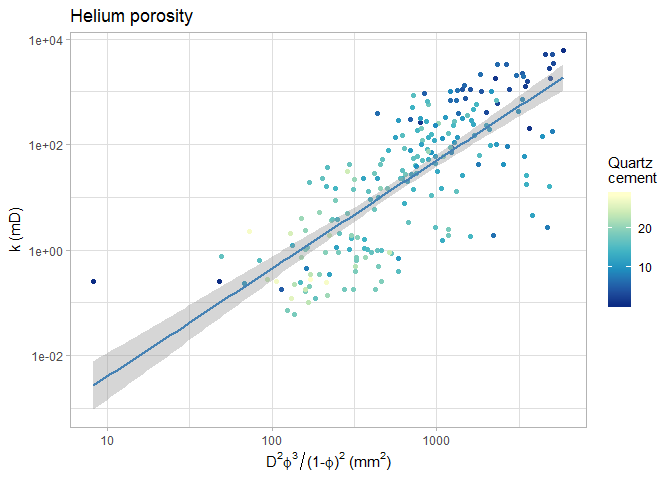
\includegraphics{garn-panda_files/figure-latex/Carman_Kozeny_unaltered-2.pdf}
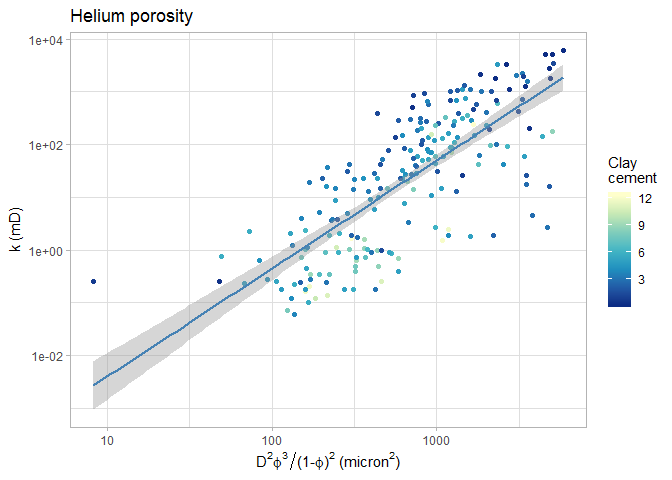
\includegraphics{garn-panda_files/figure-latex/Carman_Kozeny_unaltered-3.pdf}

\begin{verbatim}
## 
## Call:
## lm(formula = KLH ~ mean_GS^2 * POR^3/(1 - POR)^2, data = df)
## 
## Residuals:
##    Min     1Q Median     3Q    Max 
## -924.9 -304.3  -95.5  196.4 3599.4 
## 
## Coefficients:
##               Estimate Std. Error t value Pr(>|t|)    
## (Intercept) -2816.2781   364.1172  -7.735 4.20e-13 ***
## mean_GS         2.5475     0.7786   3.272  0.00125 ** 
## POR         22182.4838  2701.3698   8.212 2.16e-14 ***
## mean_GS:POR   -18.6961     6.2068  -3.012  0.00291 ** 
## ---
## Signif. codes:  0 '***' 0.001 '**' 0.01 '*' 0.05 '.' 0.1 ' ' 1
## 
## Residual standard error: 572.4 on 211 degrees of freedom
## Multiple R-squared:  0.5486, Adjusted R-squared:  0.5422 
## F-statistic: 85.49 on 3 and 211 DF,  p-value: < 2.2e-16
\end{verbatim}

\begin{verbatim}
## 
## Call:
## lm(formula = KLH ~ GS^2 * POR^3/(1 - POR)^2, data = df)
## 
## Residuals:
##    Min     1Q Median     3Q    Max 
## -950.1 -292.3  -78.4  175.1 3591.9 
## 
## Coefficients:
##              Estimate Std. Error t value Pr(>|t|)    
## (Intercept) -3282.395    428.431  -7.661 6.57e-13 ***
## GS              4.512      1.167   3.865 0.000148 ***
## POR         25144.664   3090.141   8.137 3.46e-14 ***
## GS:POR        -32.015      8.960  -3.573 0.000437 ***
## ---
## Signif. codes:  0 '***' 0.001 '**' 0.01 '*' 0.05 '.' 0.1 ' ' 1
## 
## Residual standard error: 567 on 211 degrees of freedom
## Multiple R-squared:  0.557,  Adjusted R-squared:  0.5507 
## F-statistic: 88.43 on 3 and 211 DF,  p-value: < 2.2e-16
\end{verbatim}

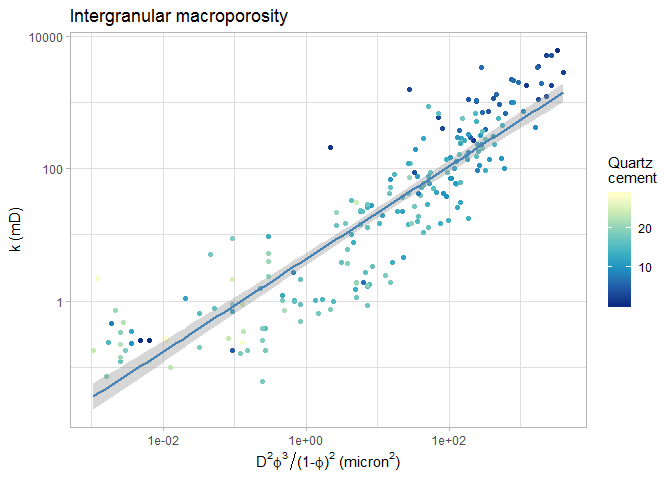
\includegraphics{garn-panda_files/figure-latex/Carman_Kozeny_unaltered-4.pdf}

\begin{verbatim}
## 
## Call:
## lm(formula = KLH ~ IMP^3/(1 - IMP)^2, data = mutate(df, IMP = IMP/100))
## 
## Residuals:
##    Min     1Q Median     3Q    Max 
## -896.7 -320.2  -11.7  258.0 3582.9 
## 
## Coefficients:
##             Estimate Std. Error t value Pr(>|t|)    
## (Intercept)  -375.27      56.98  -6.586 3.48e-10 ***
## IMP         11742.47     699.04  16.798  < 2e-16 ***
## ---
## Signif. codes:  0 '***' 0.001 '**' 0.01 '*' 0.05 '.' 0.1 ' ' 1
## 
## Residual standard error: 556.1 on 213 degrees of freedom
## Multiple R-squared:  0.5698, Adjusted R-squared:  0.5678 
## F-statistic: 282.2 on 1 and 213 DF,  p-value: < 2.2e-16
\end{verbatim}

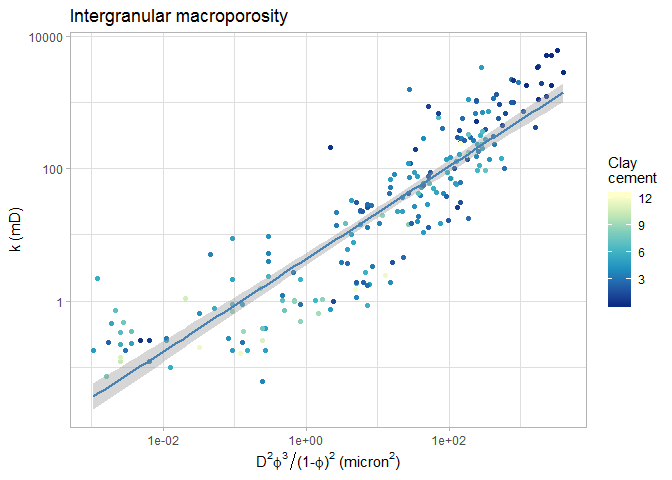
\includegraphics{garn-panda_files/figure-latex/Carman_Kozeny_unaltered-5.pdf}
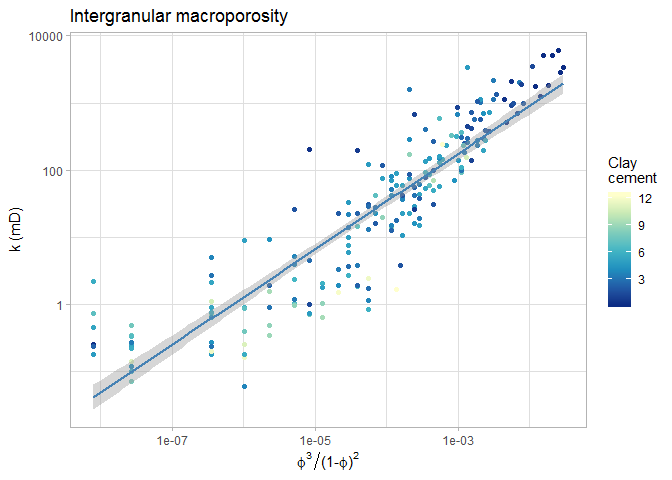
\includegraphics{garn-panda_files/figure-latex/Carman_Kozeny_unaltered-6.pdf}

\begin{verbatim}
## 
## Call:
## lm(formula = KLH ~ mean_GS^2 * IMP^3/(1 - IMP)^2, data = mutate(df, 
##     IMP = IMP/100))
## 
## Residuals:
##     Min      1Q  Median      3Q     Max 
## -1092.5  -277.2   -15.1   227.9  3510.4 
## 
## Coefficients:
##               Estimate Std. Error t value Pr(>|t|)    
## (Intercept)  -504.0130   126.0618  -3.998 8.83e-05 ***
## mean_GS         0.3472     0.2499   1.390   0.1661    
## IMP         16023.1146  2002.5738   8.001 8.09e-14 ***
## mean_GS:IMP   -10.9041     4.7369  -2.302   0.0223 *  
## ---
## Signif. codes:  0 '***' 0.001 '**' 0.01 '*' 0.05 '.' 0.1 ' ' 1
## 
## Residual standard error: 551.7 on 211 degrees of freedom
## Multiple R-squared:  0.5807, Adjusted R-squared:  0.5747 
## F-statistic:  97.4 on 3 and 211 DF,  p-value: < 2.2e-16
\end{verbatim}

\begin{verbatim}
## 
## Call:
## lm(formula = KLH ~ GS^2 * IMP^3/(1 - IMP)^2, data = mutate(df, 
##     IMP = IMP/100))
## 
## Residuals:
##     Min      1Q  Median      3Q     Max 
## -1081.6  -274.5    -5.4   217.5  3535.0 
## 
## Coefficients:
##               Estimate Std. Error t value Pr(>|t|)    
## (Intercept)  -531.8282   156.7496  -3.393 0.000826 ***
## GS              0.5262     0.4137   1.272 0.204739    
## IMP         16535.3395  2263.9842   7.304 5.65e-12 ***
## GS:IMP        -15.3380     6.8062  -2.254 0.025252 *  
## ---
## Signif. codes:  0 '***' 0.001 '**' 0.01 '*' 0.05 '.' 0.1 ' ' 1
## 
## Residual standard error: 551.7 on 211 degrees of freedom
## Multiple R-squared:  0.5807, Adjusted R-squared:  0.5747 
## F-statistic: 97.41 on 3 and 211 DF,  p-value: < 2.2e-16
\end{verbatim}


\end{document}
